\chapter{Estado del Arte}\label{ch:estado-del-arte}

La integración de la inteligencia artificial en la dermatología ha transitado de ser una promesa académica a 
constituirse en una herramienta clínica fundamental para el diagnóstico temprano del cáncer de piel y otras 
afecciones cutáneas. Sin embargo, el éxito de estos sistemas depende de la calidad, el volumen y, sobre todo, 
la representatividad de los datos utilizados en su entrenamiento. Para el proyecto DermaUH, liderado por la 
Facultad de Matemática y Computación de la Universidad de La Habana, la creación de una base de imágenes 
dermatológicas propia no representa solo un avance técnico, sino un imperativo de soberanía tecnológica, 
pertinencia epidemiológica y viabilidad económica~\cite{prensalatina_dermauh}. Este capítulo detalla 
el estado del arte de los repositorios globales y analiza exhaustivamente los factores que exigen el 
desarrollo de una infraestructura de datos soberana que refleje la realidad endémica de la población cubana.

\section{Evolución y Clasificación de los Repositorios Globales}\label{sec:repositorios-globales}

El desarrollo de algoritmos de aprendizaje profundo para la clasificación de lesiones cutáneas ha sido 
impulsado por la apertura de grandes archivos digitales. Estos repositorios han evolucionado desde 
colecciones institucionales privadas hacia plataformas masivas de acceso público que estandarizan tanto 
la imagen como los metadatos asociados.


\subsection{El Archivo ISIC: Estándar Global y sus Desafíos}\label{sec:isic}

La \textit{International Skin Imaging Collaboration} (ISIC) representa el esfuerzo más significativo a nivel 
mundial para estandarizar la imagen dermatológica y reducir la mortalidad por melanoma, así como minimizar 
las biopsias innecesarias mediante la mejora en la precisión y eficiencia del diagnóstico 
temprano~\cite{itobos_isic,isic_mission}. 

El desarrollo de la imagenología dermatológica evolucionó durante décadas sin el beneficio de estándares 
específicos para la especialidad, a diferencia de otros campos que adoptaron rápidamente protocolos como 
DICOM (\textit{Digital Image Communication in Medicine}). Esta falta de uniformidad se debió en parte a que 
la fotografía dermatológica solía realizarse con equipos convencionales, y la reciente era de la tecnología 
móvil complicó aún más la capacidad de establecer estándares técnicos que siguieran el ritmo de los cambios 
tecnológicos. Ante esto, ISIC surge como una asociación entre la academia y la industria, 
centrando su actividad en la calidad de la imagen, la protección de la privacidad de los pacientes y la 
interoperabilidad para compartir metadatos eficazmente~\cite{isic_mission}.

\begin{table}[htbp]
\centering
\caption{Estadísticas del Archivo ISIC ~\cite{isic_home} (Visitado el 4 de marzo de 2026).}\label{tab:isic-stats}
\begin{tabular}{lr}
\toprule
\textbf{Indicador} & \textbf{Cifra} \\
\midrule
Total de imágenes registradas & 1\,203\,225 \\
Imágenes de acceso público & 549\,571 \\
Usuarios registrados en la plataforma & 10\,413 \\
Publicaciones científicas generadas & 22 \\
Citaciones totales registradas & 1\,000+ \\
\bottomrule
\end{tabular}
\end{table}

\subsubsection{Funcionalidades Avanzadas para Usuarios e Investigadores}

El repositorio ISIC ofrece múltiples puntos de entrada para diferentes perfiles de usuario. 
Su extensa galería de acceso público permite a los clínicos e investigadores explorar decenas de miles de 
imágenes de alta calidad, definiendo colecciones y recopilando anotaciones para estudios específicos mediante 
filtros avanzados por diagnóstico, sitio anatómico o demografía. 

Para aquellos profesionales interesados en aportar datos de sus propias consultas, la plataforma dispone de un 
portal de carga estructurado que exige la aceptación de términos de uso y el envío de imágenes junto con 
archivos de metadatos estrictamente apegados a su diccionario oficial~\cite{isic_archive_contribute}. Resulta 
destacable que este sistema permite solicitar embargos de datos de hasta un año, facilitando a los 
investigadores la retención de exclusividad mientras esperan la publicación de sus artículos científicos.

En cuanto al manejo masivo de datos, ISIC proporciona la herramienta de línea de comandos \texttt{isic-cli}, 
la cual interactúa de manera automatizada con el archivo~\cite{isic_cli}. Esta herramienta, 
junto a librerías de Python como \texttt{isicarchive}, optimiza la preparación de entornos de inteligencia artificial 
evitando solicitudes web redundantes y acelerando el procesamiento de imágenes.~\cite{isic_pypi}.

\begin{table}[htbp]
\centering
\small
\caption{Ejemplos de funcionalidades de la herramienta \texttt{isic-cli}.}\label{tab:isic-cli}
\begin{tabular}{p{4.2cm}p{8.8cm}}
\toprule
\textbf{Comando} & \textbf{Aplicación Práctica} \\
\midrule
\texttt{isic image download images/} & Descarga masiva del archivo completo para entornos de entrenamiento de IA a gran escala. \\
\texttt{isic image download --search 'diagnosis\_3:Melanoma Invasive'} & Descarga selectiva basada en etiquetas diagnósticas de nivel~3 para investigación sobre variantes de melanoma. \\
\texttt{isic image download --search 'age\_approx: AND sex:male'} & Filtrado por variables demográficas cruzadas para estudios poblacionales. \\
\texttt{isic metadata download} & Descarga independiente de todos los metadatos en formato CSV para análisis estadístico. \\
\texttt{isic collection list} & Lista de todas las colecciones disponibles y sus identificadores únicos. \\
\bottomrule
\end{tabular}
\end{table}

\subsubsection{Estructura de Metadatos y el Diccionario de Datos v2.4}

La riqueza del archivo ISIC trasciende los píxeles de sus imágenes gracias a su esquema de metadatos estandarizado, 
regido por el \textit{ISIC Archive Data Dictionary}. Su versión~2.4 introdujo una taxonomía de sitios anatómicos 
jerárquicos, resultado de un consenso Delphi de expertos, diseñada para mejorar la interoperabilidad y el análisis de 
la distribución de lesiones.~\cite{isic_home}

Los metadatos, divididos en categorías demográficas, clínicas y técnicas, son esenciales para que los modelos 
de aprendizaje profundo incorporen el contexto del paciente que los dermatólogos utilizan instintivamente en su 
práctica.

\begin{table}[htbp]
\centering
\small
\caption{Principales variables del Diccionario de Datos ISIC v2.4.}\label{tab:isic-metadata}
\begin{tabular}{p{5.5cm}p{9.5cm}}
\toprule
\textbf{Campo} & \textbf{Descripción Técnica}\\
\midrule
\texttt{isic\_id} & Identificador único global de la imagen.\\
\texttt{patient\_id} & Identificador único anónimo del paciente.\\
\texttt{age\_approx} & Edad aproximada en el momento de la captura.\\
\texttt{sex} & Sexo biológico del paciente.\\
\texttt{anatom\_site\_general} & Ubicación anatómica.\\
\texttt{diagnosis\_confirm\_type} & Método de validación del diagnóstico.\\
\texttt{benign\_malignant} & Clasificación binaria de la lesión.\\
\texttt{mel\_thick\_mm} & Grosor de Breslow para melanomas.\\
\texttt{pixels\_x}, \texttt{pixels\_y} & Dimensiones espaciales de la imagen.\\
\bottomrule
\end{tabular}
\end{table}

% Un aspecto crítico y ampliamente debatido en la literatura reciente es la fuente de la validación del diagnóstico 
% (\texttt{diagnosis\_confirm\_type}). Mientras que las etiquetas de malignidad suelen estar confirmadas 
% histopatológicamente, muchas lesiones benignas se etiquetan únicamente mediante el consenso de 
% expertos o por seguimiento clínico. Esta dependencia de etiquetas no verificadas por biopsia introduce errores sistemáticos: 
% la precisión de redes neuronales convolucionales puede caer significativamente cuando se entrenan con etiquetas de consenso y se 
% prueban contra diagnósticos verificados por biopsia, lo que resalta la necesidad de filtrar los datos según su 
% nivel de fidelidad~\cite{pmc_label_noise}.

Más allá de sus metadatos, la naturaleza colaborativa internacional de ISIC es uno de sus mayores activos. 
Sin embargo, esta participación global evidencia una fuerte concentración en centros de excelencia europeos, 
norteamericanos y australianos. Instituciones pioneras como el \textit{Memorial Sloan Kettering Cancer Center} 
(EE.\,UU.), el Hospital Clínic de Barcelona (España), la Universidad Médica de Viena (Austria) o la 
Universidad de Queensland (Australia) han sido responsables de aportar bases de datos masivas (como HAM10000 
o BCN20000) que hoy constituyen la espina dorsal del aprendizaje automático en este 
dominio~\cite{iccs_bias_derm}.

\begin{figure}[htbp]
    \centering
    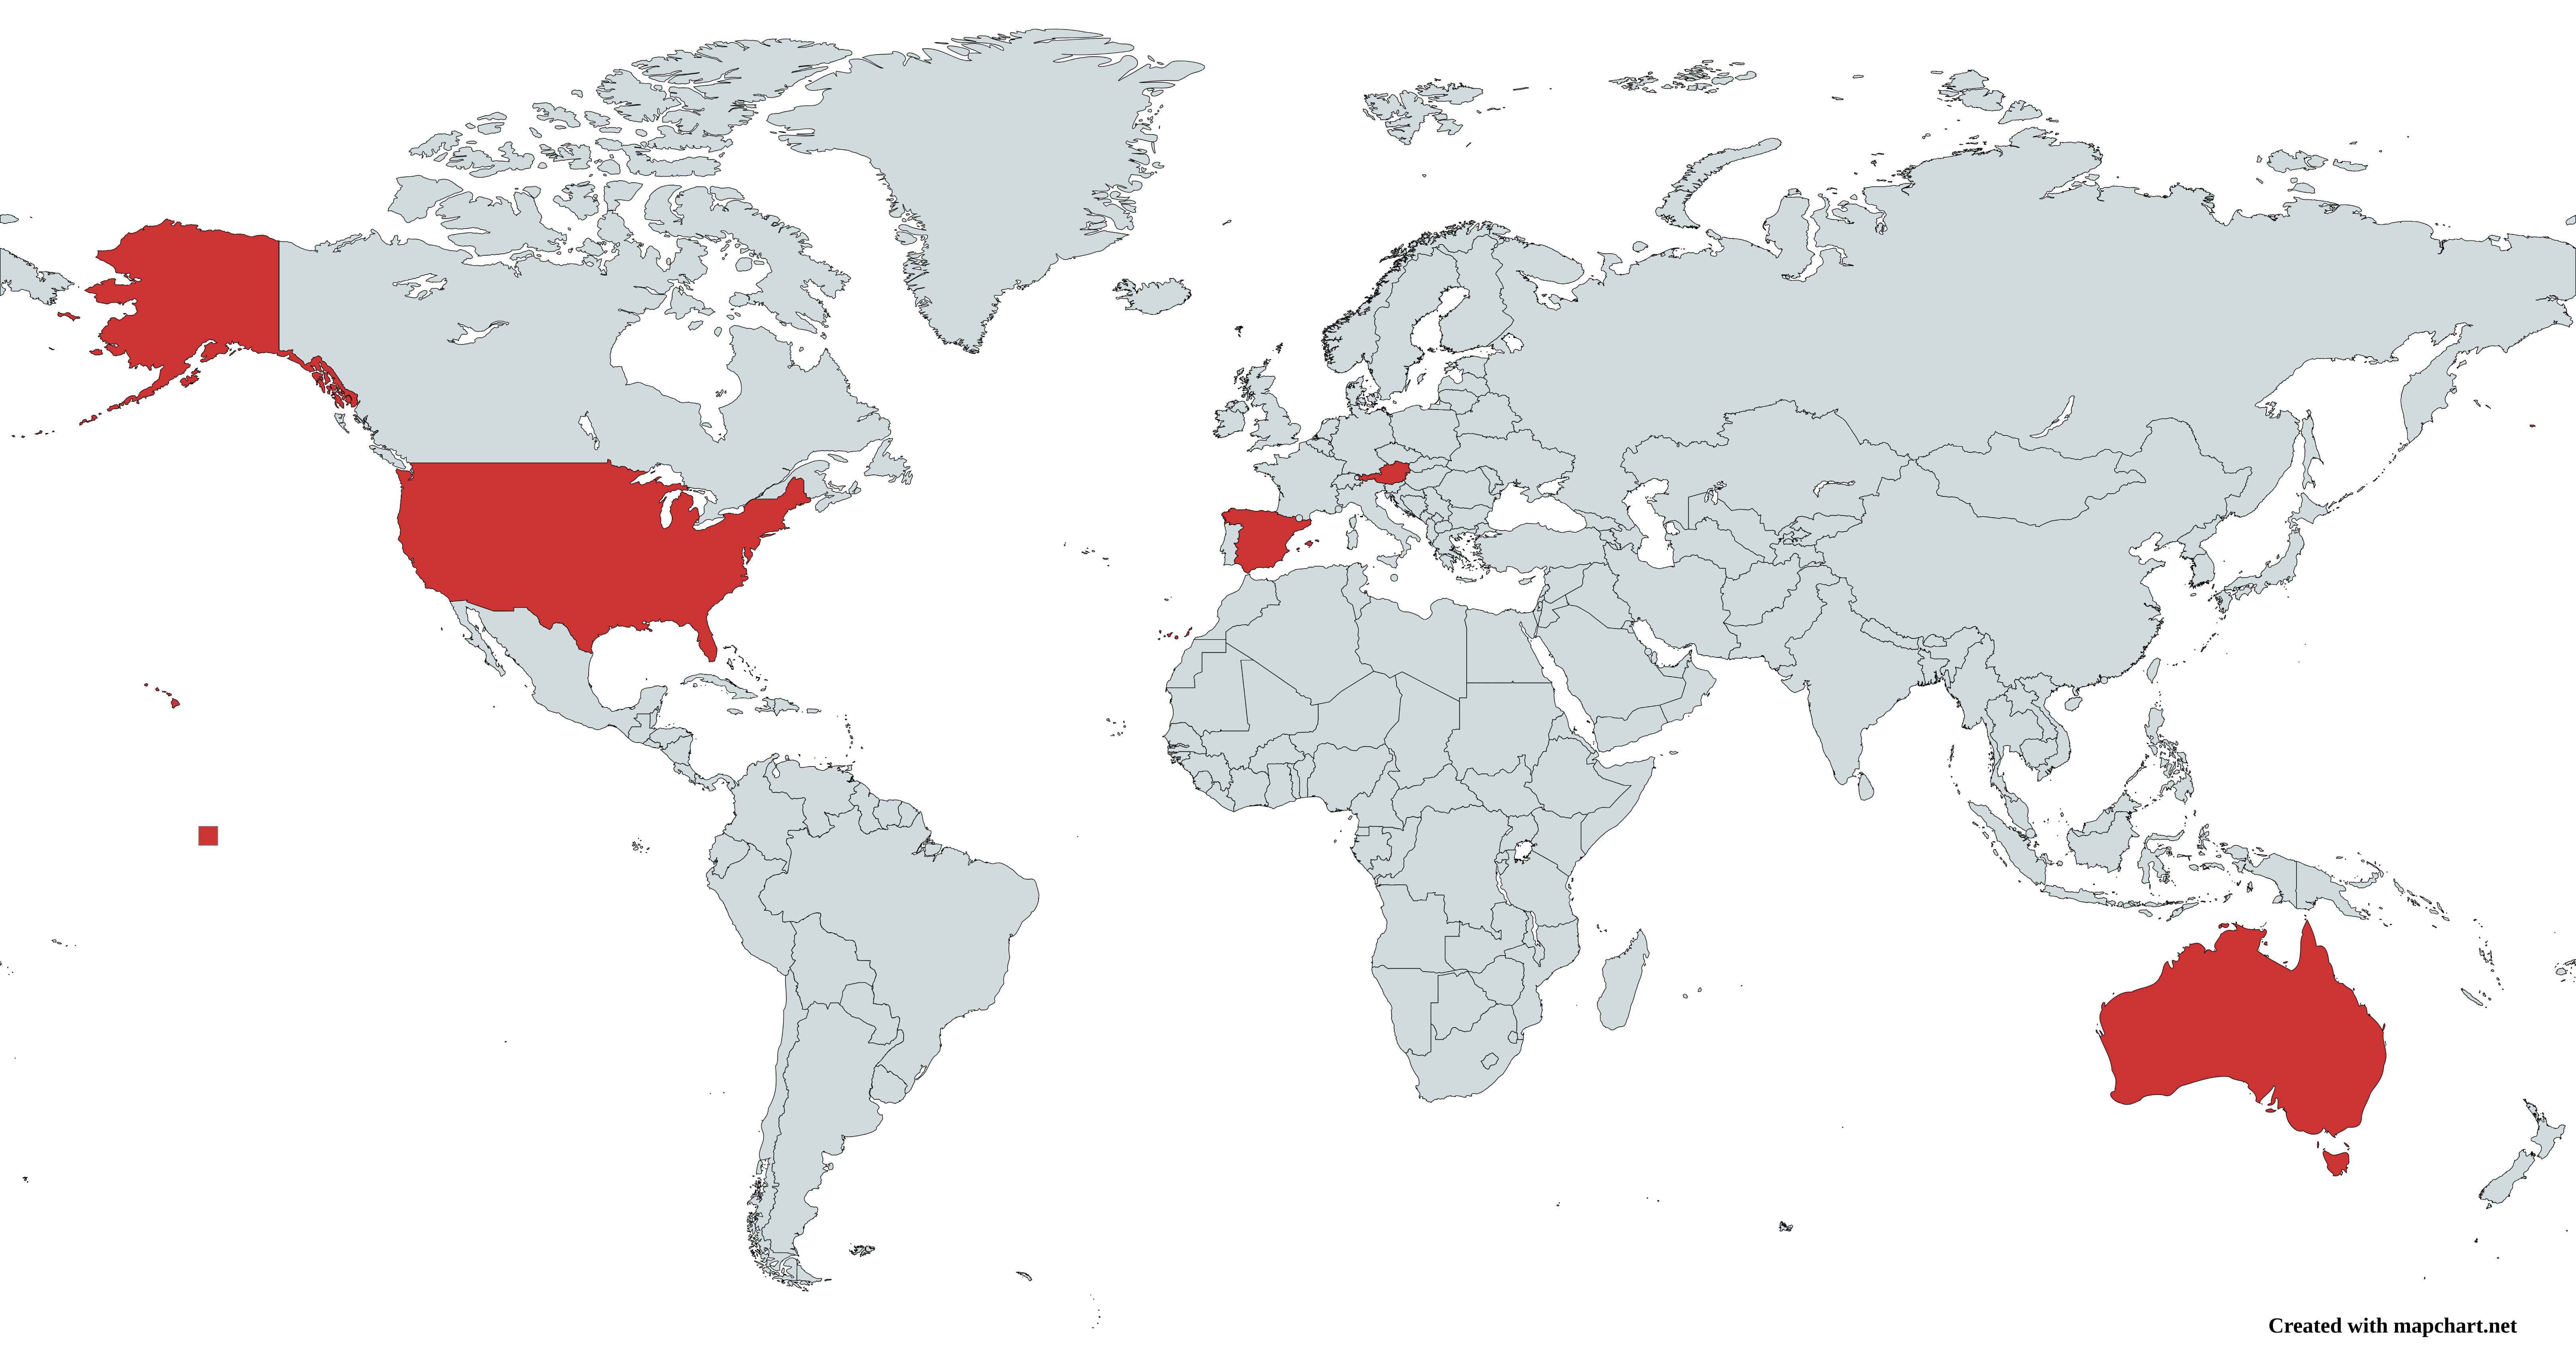
\includegraphics[width=0.75\textwidth]{Graphics/MapChart_Map.png}
    \caption{Distribución geográfica de los principales centros de investigación que contribuyen a ISIC.}
    \label{fig:isic_global_centers}
\end{figure}

El motor principal de innovación derivada de esta colaboración han sido los desafíos tecnológicos anuales. A lo 
largo de una década, estos concursos han pasado de tareas simples de segmentación en 2016 a problemas multimodales 
complejos en 2024, centrados en el diagnóstico a partir de fotografías corporales totales en 3D (3D~TBP) 
utilizando algoritmos sobre miles de imágenes de baja calidad simulando entornos de \textit{smartphones}~\cite{isic_challenge_2024_data}. 
Asimismo, se han abordado mejoras significativas en segmentación, destacando el conjunto IMA++ con más de 
17\,000 máscaras que capturan la variabilidad de anotación entre diferentes expertos~\cite{ima_plus_plus}.

A pesar de su magnitud, ISIC y los modelos derivados de él presentan limitaciones críticas que impiden una 
adopción universal sin reservas. La principal barrera es la <<brecha de generalización>>: algoritmos altamente 
precisos en el laboratorio fallan en entornos clínicos reales debido a variaciones de iluminación, enfoques o 
dispositivos~\cite{arxiv_bias_isic}. A esto se suma el problema del sesgo demográfico, 
dado que menos del 8\,\% de las imágenes en las colecciones globales representan fototipos oscuros (escalas IV 
a VI de Fitzpatrick)~\cite{iccs_bias_derm}, como se evidencia en los datos de la plataforma.

\begin{figure}[htbp]
    \centering
    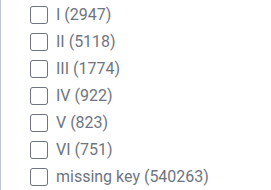
\includegraphics[width=0.45\textwidth]{Graphics/tipos_piel_isic.png}
    \caption{Distribución de fototipos de piel en el repositorio ISIC.}
    \label{fig:isic_skin_tones_raw}
\end{figure}

\begin{figure}[htbp]
    \centering
    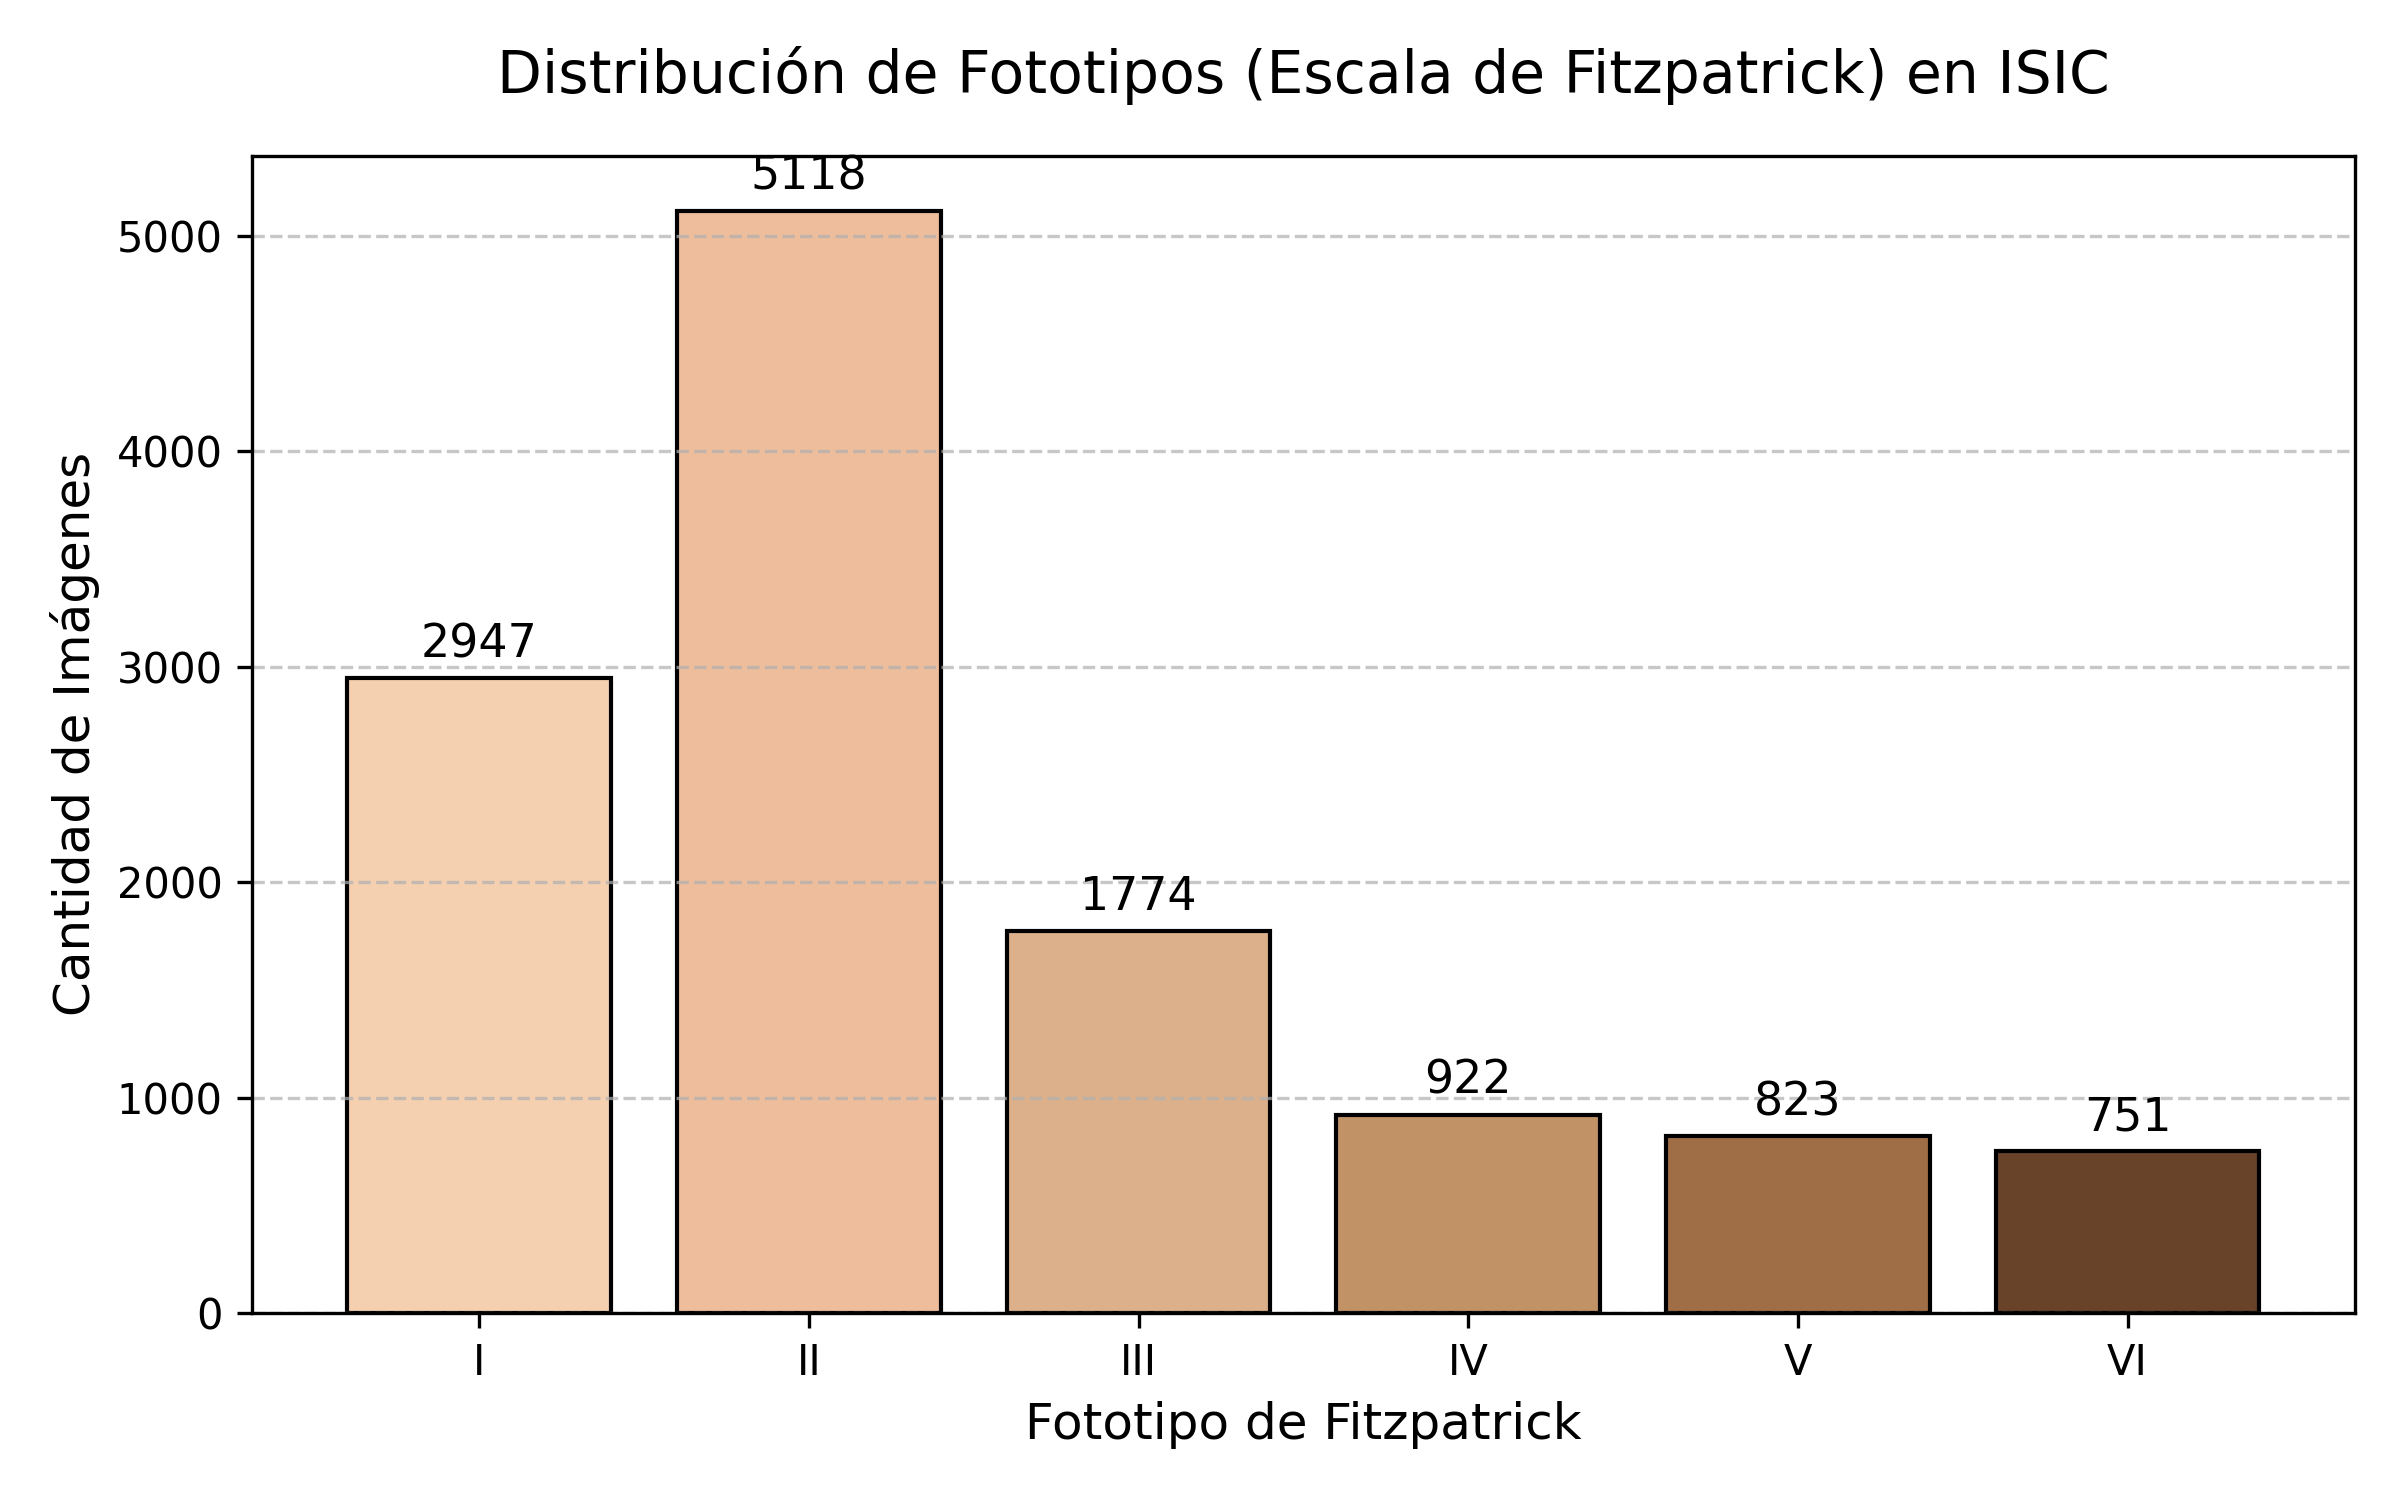
\includegraphics[width=0.8\textwidth]{Graphics/fitzpatrick_histogram.png}
    \caption{Histograma de la distribución de fototipos de piel (Escala de Fitzpatrick) en ISIC.}
    \label{fig:isic_skin_tones_hist}
\end{figure}

Esta desproporción no solo disminuye el 
rendimiento algorítmico en poblaciones con mayor pigmentación, sino que compromete la calibración de los 
sistemas, provocando que estos tiendan a sobre-diagnosticar el riesgo en nuevos conjuntos de datos, lo 
que podría conducir a un sobretratamiento perjudicial y a una profunda falta de equidad 
médica~\cite{melba_calibration}.


\subsection{El Conjunto de Datos HAM10000 y su Impacto Metodológico}\label{sec:ham10000}

El conjunto de datos \textit{Human Against Machine with 10,000 training images} (HAM10000) se ha consolidado 
como el estándar fundamental para el entrenamiento de redes neuronales convolucionales en dermatoscopia 
computacional~\cite{datasetninja_ham10000,arxiv_ham10000}. Su desarrollo fue el resultado de un esfuerzo 
sistemático de dos décadas para superar las deficiencias de repositorios más pequeños y homogéneos, 
gracias a la colaboración entre el Grupo ViDIR de la Universidad Médica de Viena (Austria) y la práctica 
dermatológica especializada en Queensland (Australia)~\cite{pmc_ham10000}. Esta dualidad proporcionó tanto 
casos clínicos hospitalarios complejos como lesiones pigmentadas comunes propias de una región con alta 
incidencia de cáncer de piel.

\subsubsection{Arquitectura de Datos y Preprocesamiento}

Para amalgamar veinte años de registros médicos, el dataset integra capturas de diversas tecnologías. 
Las diapositivas históricas fueron digitalizadas y restauradas, mientras que las adquisiciones 
contemporáneas se realizaron con dermatoscopios digitales de alta resolución (MoleMax HD). Para asegurar 
la homogeneidad visual necesaria en el aprendizaje profundo, todas las imágenes fueron filtradas 
automáticamente por un modelo \textit{InceptionV3} preentrenado para retener únicamente la visión 
dermatoscópica, normalizadas cromáticamente y redimensionadas a 800$\times$600 píxeles centrando 
la lesión~\cite{pmc_ham10000}.

El resultado final engloba 10\,015 imágenes clasificadas en siete categorías diagnósticas, que abarcan 
desde lesiones benignas prevalentes hasta neoplasias letales.

\begin{table}[htbp]
\centering
\caption{Distribución de categorías de lesión en el dataset HAM10000.}\label{tab:ham10000}
\begin{tabular}{lrl}
\toprule
\textbf{Categoría de Lesión} & \textbf{Frecuencia} \\
\midrule
Nevos melanocíticos (\texttt{nv}) & 6\,705 \\
Melanoma (\texttt{mel}) & 1\,113  \\
Queratosis benignas (\texttt{bkl}) & 1\,099 \\
Carcinoma basocelular (\texttt{bcc}) & 514  \\
Queratosis actínica (\texttt{akiec}) & 327  \\
Lesiones vasculares (\texttt{vasc}) & 142  \\
Dermatofibroma (\texttt{df}) & 115  \\
\bottomrule
\end{tabular}
\end{table}

\subsubsection{Estructura de Metadatos y Validación Semántica}

El valor clínico de HAM10000 descansa fuertemente en sus metadatos estructurados. La información asociada 
a cada imagen incluye variables demográficas y clínicas clave, como la edad (\texttt{age}), el sexo (\texttt{sex}) 
y la ubicación anatómica (\texttt{localization}). De especial importancia son los identificadores de 
lesión (\texttt{lesion\_id}), que resultan críticos metodológicamente: permiten a los desarrolladores 
aislar diferentes tomas fotográficas de una misma lesión anatómica, previniendo así la fuga de datos y 
el sobreajuste durante la partición de conjuntos de entrenamiento y prueba~\cite{arxiv_ham10000}.

Otro pilar fundamental es su jerarquía de evidencia diagnóstica (\texttt{dx\_type}). A diferencia de 
colecciones basadas puramente en consensos subjetivos, más del 50\,\% de las imágenes en HAM10000 cuentan 
con confirmación histopatológica, mientras que el resto fue verificado por seguimiento clínico 
a largo plazo, consenso de expertos o microscopía confocal~\cite{pmc_ham10000}.

\subsubsection{Análisis Crítico: Sesgos y Limitaciones del Dataset}

El ecosistema HAM10000 no se limitó a entrenar algoritmos. El consorcio acompañó la publicación con 
un extenso estudio de lectores, donde más de 113 profesionales evaluaron 
imágenes asistidos por predicciones algorítmicas e Inteligencia Artificial Explicable (XAI). 
Estos datos empíricos han posibilitado la optimización de interfaces clínico-tecnológicas que 
potencian la confianza y el juicio humano~\cite{figshare_ham10000_reader}. 

No obstante, un análisis detallado del repositorio revela contrastes significativos en su aplicabilidad 
clínica generalizada. Por un lado, sus fortalezas metodológicas son indiscutibles: la rigurosa verdad de 
campo, sustentada en una alta tasa de confirmación histopatológica, le otorga un nivel de fidelidad 
diagnóstica superior a muchos \textit{datasets} de origen colaborativo masivo. Asimismo, su enfoque 
multiclase facilita el entrenamiento de arquitecturas neuronales capaces de discriminar las siete 
lesiones pigmentadas más frecuentes, trascendiendo las limitaciones de la simple clasificación binaria. 
A esto se suma su naturaleza de código abierto, donde la disponibilidad conjunta de metadatos 
clínicos, máscaras de segmentación y herramientas de \textit{software} garantiza la reproducibilidad 
de los experimentos y su rápida adopción por la comunidad científica~\cite{github_ham10000_tools}.

A pesar de estos innegables aportes, el repositorio presenta sesgos estructurales que deben ser abordados 
con cautela. La principal deficiencia radica en su sesgo fenotípico: al carecer de metadatos explícitos 
sobre el fototipo de piel y provenir casi en su totalidad de pacientes de ascendencia 
europea (fototipos I a III de Fitzpatrick), se ha estimado una desproporción de 20:1 a favor de pieles 
claras~\cite{iccs_bias_derm}. Esta marcada asimetría compromete severamente la equidad algorítmica, propiciando fallos 
sistemáticos al diagnosticar lesiones en pieles oscuras~\cite{iccs_bias_derm}. De igual manera, se 
observa un fuerte sesgo geográfico debido a la concentración de la recolección en Australia y Austria, 
lo que restringe su validez externa en poblaciones con epidemiologías distintas, como las de América Latina 
y el Caribe~\cite{pmc_ham10000}. Finalmente, el modelo adolece de un desbalance estadístico extremo, 
dado que los nevos melanocíticos representan más del 66\,\% de la muestra, obligando a los investigadores 
a emplear técnicas avanzadas de aumento de datos para evitar que los algoritmos marginen el aprendizaje 
de patologías minoritarias pero críticas~\cite{pmc_ham10000}.


\subsection{El Conjunto de Datos PAD-UFES-20: Multimodalidad en la Salud Pública}\label{sec:pad-ufes}

La inteligencia artificial aplicada a la dermatología experimenta una transición desde modelos puramente 
visuales hacia arquitecturas multimodales que integran imágenes con historiales clínicos. 
En este paradigma, el conjunto de datos PAD-UFES-20 se erige como el protagonista indiscutible en el 
contexto latinoamericano. Desarrollado a partir del Programa de Asistencia Dermatológica de la Universidad 
Federal de Espírito Santo (Brasil), este \textit{dataset} representa un hito al reflejar la realidad 
epidemiológica y tecnológica de la salud pública, ofreciendo un modelo estructural sumamente valioso y 
cercano a la realidad médica cubana~\cite{isic_padufes,pmc_padufes}. Su naturaleza de acceso 
abierto lo convierte en un recurso estratégico para el desarrollo de tecnologías sin barreras comerciales.

\subsubsection{Construcción Social de los Datos y Características Clínicas}

El núcleo de PAD-UFES-20 consta de 2\,298 muestras fotográficas capturadas exclusivamente mediante 
teléfonos inteligentes, distribuidas en seis categorías diagnósticas, donde destaca un excepcional 
58\,\% de confirmación mediante biopsia. Sin embargo, el verdadero valor diferencial de este 
repositorio frente a otros repositorios masivos radica en su profundo archivo de metadatos asociado 
a cada lesión.~\cite{pmc_padufes}

Según los descriptores originales del \textit{dataset}, cada registro clínico puede contener hasta 
26 características estructuradas que capturan el espectro completo del paciente. Estas se pueden 
agrupar metodológicamente en:
\begin{itemize}
    \item \textbf{Demografía y Antecedentes:} Edad (\texttt{age}), sexo (\texttt{gender}), fototipo de piel (\texttt{fitzpatrick}), e historia familiar o personal de cáncer (\texttt{cancer\_history}, \texttt{skin\_cancer\_history}).
    \item \textbf{Morfología y Síntomas:} Región anatómica (\texttt{region}), diámetros de la lesión (\texttt{diameter\_1}, \texttt{diameter\_2}), presencia de dolor (\texttt{hurt}), prurito (\texttt{itch}) o crecimiento reciente (\texttt{grew}).
    \item \textbf{Factores de Riesgo y Construcción Social:} Exposición a pesticidas (\texttt{pesticide\_exposure}), tabaquismo (\texttt{smoke}) y consumo de alcohol (\texttt{drink}).
\end{itemize}

De manera sumamente innovadora, el \textit{dataset} incorpora variables de infraestructura 
habitacional, como el acceso a alcantarillado (\texttt{has\_sewage\_system}) o a agua 
corriente (\texttt{has\_piped\_water}). Estas características socioeconómicas actúan computacionalmente 
como predictores indirectos del nivel de ingresos y, por ende, del grado de 
exposición solar ocupacional o agrícola del paciente~\cite{jmir_padufes_social}. Esta amalgama de 
datos sintomáticos, antecedentes y contexto social permite a las redes neuronales emular de manera 
sin precedentes el razonamiento clínico holístico de un médico general.

A pesar de su invaluable riqueza, el repositorio no está exento de limitaciones. Adolece de un marcado 
sesgo demográfico hacia poblaciones de ascendencia europea (pomeranos), lo que reduce su 
representatividad algorítmica en fenotipos oscuros. Además, presenta una considerable variabilidad 
técnica en las imágenes, producto del uso no estandarizado de múltiples modelos de dispositivos 
móviles sin filtros automáticos de calidad en el momento de la captura~\cite{pmc_padufes}.

\subsubsection{Tecnologías Derivadas: Filtros de Calidad y Explicabilidad}

Las limitaciones técnicas de PAD-UFES-20 han servido como catalizador para el desarrollo de herramientas 
complementarias en el ámbito académico. Para abordar la variabilidad en las capturas móviles, 
han emergido \textit{frameworks} de investigación como DermAI. Este ecosistema implementa redes neuronales 
directamente en el dispositivo para actuar como un filtro de calidad en 
tiempo real, evaluando indicadores de nitidez, desenfoque y exposición antes de la inferencia clínica. 
Esto permite plantear soluciones al ruido técnico característico de las adquisiciones masivas presentes 
en PAD-UFES-20~\cite{arxiv_dermai}.

Por otro lado, para cubrir la necesidad de explicabilidad y la escasez de datos masivos, PAD-UFES-20 ha 
sido utilizado como pilar fundacional en herramientas de generación sintética como DermaSynth. Al combinar 
los ricos metadatos abiertos de PAD-UFES-20 con modelos de lenguaje de gran escala, DermaSynth ha creado 
más de 90\,000 pares de imagen y texto, dotando a la inteligencia artificial de una capacidad 
argumentativa (XAI). Es crítico destacar que, a diferencia del acceso abierto y permisivo de PAD-UFES-20, 
los modelos sintéticos derivados como DermatoLlama están estrictamente restringidos al uso académico y 
no comercial, debido a las licencias subyacentes restrictivas de los modelos corporativos utilizados para 
su creación. Así, PAD-UFES-20 no solo funciona como un repositorio primario 
fundamental, sino como el cimiento de código abierto sobre el cual se construyen y evalúan las nuevas 
arquitecturas de triaje dermatológico.


\subsection{BCN20000: Lesiones en Entornos Clínicos Reales}\label{sec:bcn20000}

La transición de la dermatología digital desde imágenes controladas de laboratorio hacia capturas en 
condiciones hospitalarias reales marca un punto de inflexión en la aplicabilidad clínica de la inteligencia 
artificial. El \textit{dataset} BCN20000 surge precisamente para afrontar este desafío. Este repositorio 
monumental fue desarrollado gracias a una colaboración multidisciplinaria de vanguardia que incluyó al 
Hospital Clínic de Barcelona, la Universitat Politècnica de Catalunya, el Memorial Sloan Kettering 
Cancer Center en Nueva York y el equipo de IBM \textit{Research AI}~\cite{scidata_bcn20000}. 

\subsubsection{Características Generales y Metadatos}

En términos de características generales, el archivo consta de 18\,946 imágenes dermatoscópicas de alta 
resolución correspondientes a 5\,583 lesiones únicas, recolectadas sistemáticamente durante un periodo de 
seis años (2010-2016) mediante múltiples dispositivos y cámaras. Esta estructura jerárquica resulta 
metodológicamente fundamental, ya que al disponer de varias capturas de un mismo objetivo anatómico, 
los investigadores pueden entrenar redes neuronales robustas previniendo la fuga de 
datos o \textit{data leakage}~\cite{arxiv_bcn20000,scidata_bcn20000}. 

Para potenciar su utilidad, cada captura está vinculada a un riguroso archivo de metadatos que proporciona 
un contexto clínico esencial. Los descriptores incluyen variables demográficas clásicas, como la edad y 
el sexo del paciente, además de información clínica vital que comprende la ubicación anatómica primaria, 
la fecha exacta de captura y el diagnóstico definitivo, el cual está avalado mayoritariamente por escrutinio 
histopatológico. La disponibilidad de identificadores trazables explícitos (\texttt{lesion\_id}) cierra 
el cerco de su solidez técnica~\cite{scidata_bcn20000}.

\subsubsection{Desafíos Clínicos, Deficiencias y Sesgos Estructurales}

El verdadero aporte científico del BCN20000 radica, paradójicamente, en las ``deficiencias'' técnicas 
intencionadas que incorpora, enmarcadas en su filosofía de recolección \textit{in the wild} (en estado salvaje). 
A diferencia de repositorios anteriores altamente curados y estéticos, este \textit{dataset} refleja el 
caos visual de la consulta diaria. Obliga a los algoritmos a lidiar con una notable complejidad anatómica 
y de escala, incluyendo localizaciones difíciles como uñas y mucosas, así como lesiones cuyo tamaño supera 
la apertura focal del dermatoscopio. Además, preserva de manera deliberada el ruido clínico, presentando 
imágenes ocluidas por vello corporal, burbujas de gel de contacto o marcas quirúrgicas con rotulador, 
lo que exige técnicas de inferencia avanzadas para evitar que la inteligencia artificial aprenda correlaciones 
espurias~\cite{scidata_bcn20000}.

Para mitigar los fallos predictivos en escenarios atípicos, los arquitectos del repositorio innovaron al 
incluir una categoría diagnóstica adicional etiquetada como ``fuera de distribución'' (OOD, por sus siglas en inglés). 
Esta clase agrupa alteraciones que no encajan en los diagnósticos principales, enseñando al modelo a 
identificar lo ``desconocido'' en lugar de forzar un falso positivo. A pesar de su exhaustivo realismo, 
la base de datos no está exenta de deficiencias sistémicas indeseadas. Al haberse recolectado íntegramente 
en un único centro de España, exhibe un severo sesgo geográfico e infra-representación de tonos de piel 
oscuros (centrándose en fototipos I a III de Fitzpatrick). Esta carencia estructural compromete de manera 
sustancial su equidad algorítmica y su viabilidad como fuente única de entrenamiento para su despliegue 
seguro en poblaciones con mayor diversidad fenotípica~\cite{arxiv_bcn20000}.

\subsection{Derm7pt: Multimodalidad y Arquitecturas de IA Explicable}\label{sec:derm7pt}

A diferencia de los repositorios masivos que priorizan el volumen de imágenes, el conjunto de datos Derm7pt 
se centra en la riqueza cualitativa y el soporte al razonamiento clínico. Su diseño pivota íntegramente sobre 
el \textit{Checklist} de 7 Puntos de Argenziano, un algoritmo médico formal establecido para la detección de 
melanoma que evalúa la presencia de criterios mayores (ej. red de pigmento atípica, velo azul-blanquecino) y 
menores (ej. estrías irregulares). Esta base de datos proporciona más de 2\,000 imágenes clínicas y 
dermatoscópicas pareadas para 1\,011 casos, consolidando un entorno propicio para la Inteligencia Artificial 
Explicable (XAI)~\cite{github_derm7pt,arxiv_derm7pt_concept}.

La arquitectura de datos de Derm7pt destaca por su multimodalidad y altísima granularidad conceptual. Cada 
imagen está etiquetada no solo con uno de los 19 diagnósticos específicos posibles, sino con la presencia 
individual de cada concepto biológico del \textit{Checklist}. Adicionalmente, incluye metadatos clínicos poco 
comunes, destacando la ``elevación'' de la lesión (plana, palpable o nodular) y el nivel de dificultad 
diagnóstica percibido por el experto. Estas anotaciones a nivel de concepto permiten entrenar Modelos de 
Cuello de Botella Conceptual (\textit{Concept Bottleneck Models}), donde la red neuronal emite su diagnóstico 
justificándolo expresamente a través de las características visuales detectadas, proporcionando una cadena de 
razonamiento clínico directamente auditable por el especialista médico~\cite{arxiv_derm7pt_concept}.

A pesar de ser una herramienta invaluable para la transparencia algorítmica, Derm7pt presenta limitaciones 
inherentes a su tamaño. Su reducida escala genera un desequilibrio de clases extremo que complica el 
entrenamiento sin técnicas de generación sintética. Adicionalmente, investigaciones en el campo de la 
teoría de conjuntos han demostrado que existe una ``inconsistencia conceptual'' en su etiquetado, donde 
combinaciones idénticas de características visuales conducen ocasionalmente a diagnósticos clínicos 
opuestos, imponiendo un límite teórico insalvable de precisión matemática para los modelos estrictamente 
conceptuales~\cite{arxiv_derm7pt_concept}. No obstante, Derm7pt sigue marcando el estándar fundamental en 
la intersección entre la clasificación por aprendizaje profundo y la práctica médica basada en la evidencia.


\section{El Problema del Sesgo Demográfico y la Necesidad de Datos Endémicos}\label{sec:sesgo-demografico}

La eficacia de un sistema de diagnóstico por imagen asistido por inteligencia artificial está 
estrictamente condicionada por la similitud estadística entre la distribución de sus datos de 
entrenamiento y la población clínica a la que se aplica. El fenómeno conocido como \textit{Domain Shift} 
(cambio de dominio) establece que cuando un algoritmo se enfrenta a datos fuera de su distribución 
original, su rendimiento se degrada de forma acentuada. Estudios recientes han demostrado que modelos 
dermatológicos de vanguardia, que alcanzan precisiones superiores al 90\,\% en entornos controlados, 
experimentan caídas de hasta un 30\,\% en su sensibilidad al ser evaluados en poblaciones con fenotipos 
distintos o con condiciones de captura no estandarizadas~\cite{sciadv_daneshjou2022,arxiv_kinyanjui2019}. 
En el caso particular de Cuba, la adopción directa de repositorios internacionales falla en dos 
dimensiones epidemiológicas críticas: la distribución del fototipo de piel y el espectro de patologías 
endémicas.


\subsection{La Escala de Fitzpatrick y la Brecha de Equidad}\label{sec:fitzpatrick}

La dermatología académica ha utilizado históricamente la escala de Fitzpatrick (tipos I al VI) para 
clasificar la respuesta de la piel a la radiación ultravioleta y su nivel de pigmentación constitutiva. 
A partir del análisis exhaustivo realizado en las secciones anteriores sobre los 
principales \textit{datasets} globales, es evidente que la inteligencia artificial hereda una brecha 
sistémica de equidad. Repositorios de referencia como HAM10000 y BCN20000, al ser recolectados casi 
íntegramente en clínicas de Austria, Australia y España, presentan una desproporción a favor de fenotipos 
claros (Fitzpatrick I-III) frente a fenotipos oscuros (IV-VI)~\cite{pmc_ham10000,arxiv_bcn20000}. 
Incluso iniciativas concebidas en el Sur Global, como PAD-UFES-20 en Brasil, demostraron arrastrar 
sesgos inherentes hacia poblaciones con ascendencia europea~\cite{pmc_padufes}.

\begin{figure}[htbp]
    \centering
    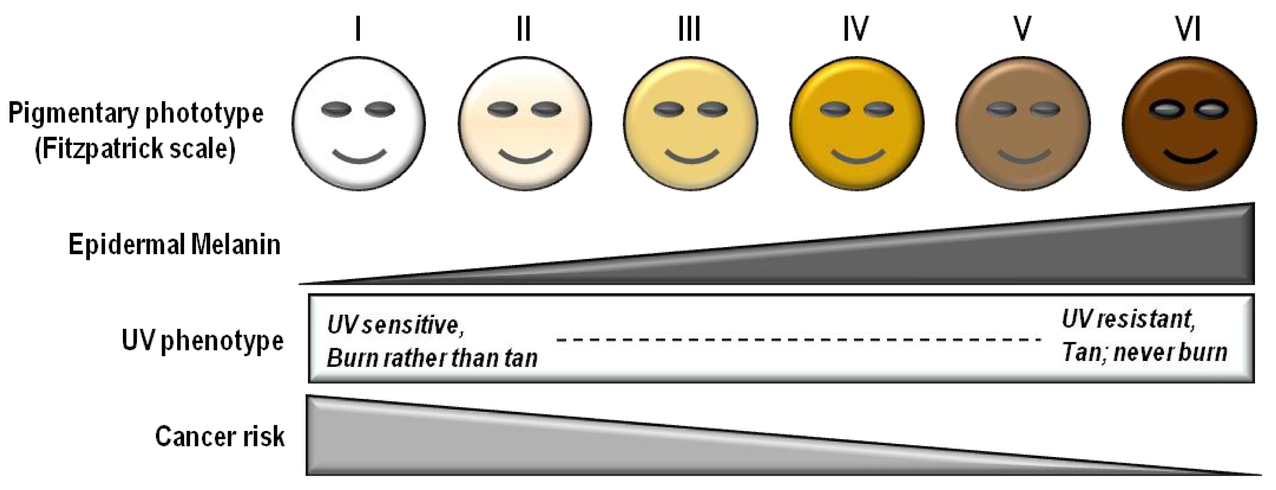
\includegraphics[width=0.85\textwidth]{Graphics/Piel-cancer-tonos.png}
    \caption{Manifestación visual de lesiones cutáneas a través de diferentes tonos de piel.}
    \label{fig:piel_tonos_cancer}
\end{figure}

Esta marginación estructural genera modelos algorítmicamente sesgados. Las redes neuronales entrenadas 
predominantemente en pieles claras exhiben una disminución marcada en su rendimiento y equidad diagnóstica 
cuando se enfrentan a pieles oscuras o mestizas. En pieles con alta concentración de melanina, 
patologías críticas como el melanoma a menudo se presentan sin la clásica red de pigmento oscuro 
visible en caucásicos, manifestándose de formas atípicas o en localizaciones acrales (palmas y plantas) 
que están sistemáticamente subrepresentadas en las bases de datos abiertas~\cite{sciadv_daneshjou2022}.

\begin{table}[htbp]
\centering
\caption{Escala de Fitzpatrick y representación en datasets globales (ISIC, HAM10000, PAD-UFES-20, Derm7pt).}\label{tab:fitzpatrick}
\begin{tabular}{clp{5.5cm}}
\toprule
\textbf{Tipo} & \textbf{Descripción Fenotípica} & \textbf{Representación en Datasets} \\
\midrule
I & Piel muy clara, siempre se quema & Sobrerrepresentado ($>$45\,\% en ISIC)~\cite{iccs_bias_derm} \\
II & Piel clara, suele quemarse & Sobrerrepresentado~\cite{iccs_bias_derm} \\
III & Piel clara a oliva, broncea gradualmente & Moderada~\cite{arxiv_skin_tone} \\
IV & Piel morena, broncea con facilidad & Escasa~\cite{arxiv_skin_tone} \\
V & Piel morena oscura, broncea oscuro & Críticamente baja ~\cite{arxiv_skin_tone} \\
VI & Piel negra, nunca se quema & Casi inexistente ($<$1\,\%)~\cite{iccs_bias_derm} \\
\bottomrule
\end{tabular}
\end{table}

En Cuba, la realidad demográfica está definida por un alto grado de mestizaje, resultando en una 
prevalencia epidemiológica sumamente significativa de fototipos III, IV y V. La importación y uso 
directo de herramientas algorítmicas entrenadas en el extranjero, sin un ajuste 
fino (\textit{fine-tuning}) sobre datos locales, no solo resulta ineficiente, sino que éticamente 
podría conducir a errores diagnósticos sistemáticos y agravar las disparidades en la atención 
médica en el país.


\section{Motivos Económicos}\label{sec:motivos-economicos}

La creación de una base de datos nacional no es solo una cuestión de precisión médica, sino de viabilidad 
financiera y supervivencia estratégica ante las restricciones externas. Para dimensionar adecuadamente 
esta afirmación, es necesario contrastar la realidad salarial del profesional cubano con los costos 
internacionales que implica el desarrollo de infraestructuras de inteligencia artificial en el 
ámbito dermatológico.


\subsection{Realidad Salarial del Profesional Cubano}\label{sec:salario-cubano}

Según la publicación oficial \textit{Salario Medio en Cifras. Cuba 2025} de la Oficina Nacional de 
Estadística e Información (ONEI), el salario medio mensual del sector estatal en Cuba durante el año 
2025 se situó en 6\,930 pesos cubanos (CUP)~\cite{onei_salario_2025}. En el sector de la salud pública, el 
salario medio mensual estuvo incluso por debajo de la media general, situándose en 6\,635~CUP~\cite{onei_salario_2025}.

Un aspecto crítico para contextualizar estas cifras es su equivalencia en divisas. Al tipo de cambio 
del mercado informal ---que es el referente real para la adquisición de bienes e insumos en la 
isla---, el salario medio nacional de 6\,930~CUP equivale actualmente a 10~USD mensuales aproximadamente~\cite{el_toque_exchange_rates}. 
Esto significa que un profesional de la salud, 
cuyo salario escala es de 6\,635~CUP, percibe un ingreso mensual inferior a 10~USD al tipo de cambio 
real. Incluso considerando los pagos complementarios por antigüedad (entre 1\,000 y 3\,000~CUP 
adicionales), guardias médicas y categorías docentes o científicas, el ingreso total de un especialista 
rara vez supera los 25~USD mensuales.


\subsection{Costos Internacionales de Anotación y Curación de Datos}\label{sec:etiquetado}

El desarrollo de una base de datos propia permite optimizar el uso de los recursos humanos especializados del 
país. El etiquetado de imágenes médicas es una tarea de alta complejidad que requiere la participación de 
dermatólogos expertos~\cite{datavlab_annotation,medrxiv_preannotation}. En el mercado internacional, la 
anotación especializada de imágenes dermatológicas presenta costos que resultan prohibitivos 
cuando se contrastan con la capacidad adquisitiva cubana.

Las tarifas publicadas por proveedores internacionales de anotación ilustran esta realidad. La plataforma 
GetAnnotator, por ejemplo, ofrece planes de suscripción mensual para anotadores dedicados, donde el plan 
\textit{Expert} ---el único recomendado para anotación médica, que incluye personal con más de 4 años de 
experiencia--- tiene un costo de 899~USD mensuales por anotador~\cite{getannotator_pricing}. Según 
AnnotationBox, las tarifas por imagen para segmentación semántica oscilan entre 0,50 y 3,00~USD por 
imagen~\cite{annotationbox_pricing}.

\begin{table}[htbp]
\centering
\small
\caption{Costos internacionales de anotación de imágenes médicas para IA (2024--2025).}\label{tab:costos-anotacion}
\begin{tabular}{p{6.5cm}r}
\toprule
\textbf{Concepto} & \textbf{Costo (USD)} \\
\midrule
Anotación por imagen (clasificación básica)~\cite{annotationbox_pricing} & 0,02 -- 0,20 \\
Anotación por imagen (segmentación semántica)~\cite{annotationbox_pricing} & 0,50 -- 3,00 \\
Anotador experto médico (plan mensual)~\cite{getannotator_pricing} & 899/mes \\
\bottomrule
\end{tabular}
\end{table}

Para ilustrar la magnitud de esta brecha, considérese un escenario conservador: la curación de un 
\textit{dataset} de apenas 5\,000 imágenes dermatológicas con anotación experta de segmentación 
a un costo medio de 1,50~USD por imagen representaría un gasto de 7\,500~USD, sin incluir la 
revisión por un dermatólogo certificado. Esta cifra equivale 
aproximadamente a \textbf{62 años de salario} de un profesional de la salud cubano.

Cuba, sin embargo, cuenta con una red de hospitales y especialistas que pueden generar este conocimiento 
como parte de su práctica clínica e investigativa, eliminando la necesidad de importar estos servicios 
de anotación~\cite{fundacionuh_taller}. Al integrar el etiquetado de imágenes dentro del flujo de 
trabajo habitual de los dermatólogos del sistema nacional de salud, el proyecto DermaUH transforma un 
costo operativo que sería inalcanzable en divisas en una inversión de capital humano ya existente, 
aprovechando la fortaleza del modelo de salud pública cubano~\cite{pmc_ciencia_innovacion_cuba}.


\subsection{Inviabilidad Económica de la Dependencia Tecnológica Externa}\label{sec:inviabilidad-economica}

Más allá del etiquetado, el ciclo completo de desarrollo de inteligencia artificial para dermatología 
involucra costos de infraestructura computacional sustanciales. El entrenamiento de modelos de 
aprendizaje profundo en plataformas comerciales de computación en la nube requiere instancias con 
unidades de procesamiento gráfico (GPU) de alto rendimiento. Según las páginas oficiales de precios 
de los principales proveedores, las tarifas bajo demanda (\textit{on-demand}) por hora de GPU 
para entrenamiento de modelos oscilan entre 5 y 98~USD dependiendo de la arquitectura de 
\textit{hardware}: una instancia \texttt{p5.4xlarge} con una GPU NVIDIA H100 en Amazon Web Services 
cuesta aproximadamente 6,88~USD/hora~\cite{aws_ec2_pricing}; una instancia A2 con GPU NVIDIA A100 
en Google Cloud se sitúa en torno a 5~USD/hora~\cite{gcp_gpu_pricing}; y la serie 
\texttt{ND H100 v5} de Microsoft Azure alcanza los 98,32~USD/hora para una configuración 
completa de 8~GPUs~\cite{azure_gpu_pricing}. Un proyecto de desarrollo completo, 
incluyendo experimentación, entrenamiento y validación, puede requerir cientos o miles de horas 
de cómputo GPU, generando presupuestos de decenas de miles de dólares solo en 
infraestructura~\cite{aws_ec2_pricing,gcp_gpu_pricing}.

En un contexto donde la adquisición de insumos médicos básicos resulta ya comprometida, destinar divisas 
escasas a la contratación de servicios internacionales de anotación de datos o al alquiler de 
infraestructura de cómputo en la nube resulta económicamente inviable.

Estas comparaciones evidencian que la estrategia de desarrollar una base de datos propia, aprovechando 
los recursos humanos y la infraestructura hospitalaria existentes en el sistema nacional de salud, no 
es simplemente una opción preferible, sino la única vía económicamente viable para que Cuba participe 
de forma soberana en la revolución de la inteligencia artificial aplicada a la 
dermatología~\cite{pmc_ciencia_innovacion_cuba,scielosp_ciencia_cuba}.


% Puede estar en la tesis pero no aqui por ahora.
% \section{Perfil Epidemiológico: Patologías Comunes y Tropicales Desatendidas}\label{sec:perfil-epidemiologico}

% Una base de datos propia permite que DermaUH responda a las necesidades reales de morbilidad del país, y 
% no solo a las prioridades de los sistemas de salud de países desarrollados, que a menudo se limitan al 
% melanoma maligno.


% \subsection{Cáncer de Piel No Melanoma (CPNM) en Cuba}\label{sec:cpnm}

% Aunque el melanoma es más letal, el CPNM (carcinomas basocelulares y espinocelulares) es el que genera la 
% mayor carga de morbilidad en la población cubana debido a la exposición solar 
% crónica~\cite{redalyc_epidem_cancer_piel}.

% \begin{table}[htbp]
% \centering
% \caption{Principales patologías de cáncer de piel no melanoma en Cuba.}\label{tab:cpnm}
% \begin{tabular}{p{3.5cm}p{4cm}p{5cm}}
% \toprule
% \textbf{Patología} & \textbf{Importancia en Cuba} & \textbf{Contexto Local} \\
% \midrule
% Carcinoma Basocelular & 80\,\% de los casos & Alta prevalencia en mayores de 60 años~\cite{redalyc_epidem_cancer_piel} \\
% Carcinoma Espinocelular & 20\,\% de los casos & Relacionado con ocupaciones al aire libre~\cite{redalyc_epidem_cancer_piel,revfinlay_factores_riesgo} \\
% \bottomrule
% \end{tabular}
% \end{table}

% La incidencia de estas enfermedades es particularmente alta en provincias como Las Tunas y Villa Clara, 
% con tasas que superan los 55 casos por cada 100\,000 
% habitantes~\cite{redalyc_epidem_cancer_piel,revfinlay_factores_riesgo}. Un \textit{dataset} propio que 
% incluya imágenes de estas lesiones en diferentes estadios permitiría entrenar modelos de triaje para la 
% atención primaria de salud (APS), donde el médico de la familia es el primer contacto del 
% paciente~\cite{dialnet_sis_cuba,scielo_morbilidad_derm}.

\section{Estrategia de Implementación y Originalidad Científica}\label{sec:estrategia}

La creación de una base de imágenes dermatológicas cubana otorga al proyecto DermaUH una ventaja competitiva 
y científica significativa.


\subsection{Originalidad e Innovación Universitaria}\label{sec:originalidad}

En el ámbito de la investigación científica, la originalidad es un factor clave para la publicación en 
revistas de alto impacto y la obtención de patentes~\cite{anuies_investigacion,wipo_investigacion_publica}. 
Al generar datos propios que capturen el mestizaje y la patología tropical, la Universidad de La Habana no 
solo <<consume>> tecnología, sino que produce conocimiento nuevo y útil para otros países del 
Sur Global~\cite{wipo_investigacion_publica,scielosp_ciencia_cuba}. Este enfoque de <<ciclo cerrado>> 
(investigación-desarrollo-aplicación) es una prioridad de la política científica nacional para 
sustituir importaciones y exportar servicios de alto valor agregado~\cite{pmc_ciencia_innovacion_cuba,scielosp_ciencia_cuba}.


\section{Conclusiones del Capítulo}\label{sec:conclusiones-cap1}

El análisis del estado del arte y de las condiciones específicas del entorno cubano demuestra que la creación 
de una base de imágenes propia para el proyecto DermaUH es una decisión estratégica fundamentada en razones 
técnicas, económicas y éticas insoslayables.

La Tabla~\ref{tab:comparativa-repositorios} resume las características principales de los repositorios internacionales analizados en este capítulo, evidenciando las fortalezas y brechas fenotípicas que justifican la necesidad de una base de datos nacional.

\begin{table}[htbp]
\centering
\small
\caption{Comparativa de los repositorios dermatológicos internacionales analizados.}\label{tab:comparativa-repositorios}
\begin{tabular}{p{2.5cm}rp{3.5cm}p{6cm}}
\toprule
\textbf{Repositorio} & \textbf{Imágenes} & \textbf{Fototipos (Escala Fitzpatrick)} & \textbf{Características y Metadatos Destacados} \\
\midrule
ISIC Archive & >500\,000 & Principalmente I--III & Archivo global masivo. Fuerte sesgo fenotípico hacia pieles claras. \\
HAM10000 & 10\,015 & Principalmente I--III & Alta confirmación histopatológica. Metadatos de edad, sexo y localización anatómica. Limitado a 7 clases diagnósticas. \\
PAD-UFES-20 & 2\,298 & I--VI (sesgo europeo local) & Capturas exclusivas con teléfonos inteligentes. 26 variables estructuradas, incluyendo contexto socioeconómico. \\
BCN20000 & 18\,946 & Principalmente I--III & Imágenes de entorno clínico real con ruido visual y oclusiones. Incluye categoría fuera de distribución (OOD). \\
Derm7pt & >2\,000 & Principalmente I--III & Mapeo explícito con el \textit{Checklist} de 7 Puntos. Ideal para Inteligencia Artificial Explicable (XAI). \\
\bottomrule
\end{tabular}
\end{table}

La dependencia de fuentes externas no solo compromete la precisión del diagnóstico por la falta de 
representatividad fenotípica y epidemiológica, sino que también vulnera la soberanía tecnológica del país. 
Un repositorio nacional, rico en imágenes de pieles mestizas y afecciones endémicas, permitirá a Cuba 
desarrollar una herramienta adaptada a su realidad social.

Finalmente, este esfuerzo fortalece el vínculo entre la universidad y el sistema de salud, transformando 
la investigación básica en aplicaciones prácticas que mejoren la calidad de vida de la población y 
aseguren que la transformación digital de la medicina cubana sea, ante todo, soberana y equitativa.

